% ---- tnf_paper.tex lines 5848-6208: How a comparison fails while every measurement in it is correct ----
\section{How a comparison fails while every measurement in it is correct}
\label{sec:selfcheck}

Comparing number formats is harder than measuring them, and the two failures
are independent: nearly every difficulty encountered in this work left the
measurement intact and broke the comparison around it. The regularities below are
stated because they generalise past this subject, and because every quantitative
claim in this paper rests on having ruled them out. They are the conditions under
which a ratio between two formats means anything at all.

\paragraph{On what is being compared.} A ratio is meaningful only if both sides
were built as their own advocate would build them; seven times here a ratio
changed sign or magnitude when the other side was rebuilt
(\extended{the scale-applier section}). Systems whose range scales differently with
width, one exact and one approximate, have no storage-matched ratio at all --- a
quantity depending on an unstated choice has no limit and cannot converge, which
is why six successive instrument corrections failed to settle one number. Where
one system's figure of merit is constant in a parameter and another's varies in
it, the well-posed comparison is a crossover and not a verdict
(the taper-delay theorem and \extended{the crossover section}), and such a
crossover is an assertion about the workload rather than about the formats.

\paragraph{On the instrument.} Under placement-seed variation LUT count is
invariant and achieved frequency moves by $11.4\%$, so any metric combining them
inherits the timing variance in full, and a ranking resolves only rows separated
by more than that. A ratio over correlated factors restates the dominant one: on
the combined harness, ranking by throughput per area reproduced ranking by
$1/\text{area}$ at a Spearman correlation of $0.961$. And a result that moves the
same way under every successive correction is still moving.

\paragraph{On the harness.} Three defects appeared in the synthesis harness, none
visible in any number, each changing a headline by 10 to 50 percent; a second,
software harness contributed three more of its own, recorded in
\extended{the applicability section}, so the total across both is six. A component shared by every
candidate is a confound rather than a constant, because it leaves area
differences intact and delay differences not. A harness observing part of a
design's output prunes each candidate in proportion to \emph{its own} output
width --- observing four bits of a 32-bit datapath left 27 LUTs of 179 while
leaving an adjacent 6-bit design nearly whole. And net-of-harness subtraction
requires the harness to be present in full in every build, since a design
consuming fewer of its sources prunes the rest.

\paragraph{On sources.} A defect found in an abstract is a hypothesis: abstracts
compress, and compression is indistinguishable from omission. An aggregated
search result may combine claims from several papers into wording present in
none. Both external criticisms we raised during this work dissolved on contact
with the papers themselves.


\paragraph{What this is worth.} Applied to two external papers read in full the
procedure produced no findings against them, and on both occasions caught our own
reading of them instead. We
therefore describe it as an instrument for checking one's own work, and not as a
method for auditing anyone else's. Three of the checks are mechanised as gates in
continuous integration; the full statement is in the accompanying note.





\subsection{Figures whose generating data is not in the repository}
\label{sec:provenance}
Twenty claims were withdrawn during this work, and a withdrawn claim's number
does not remove itself from a paper. A traceability check
(\texttt{tools/\allowbreak check\_\allowbreak paper\_\allowbreak numbers.py}) extracts every distinctive numeric
literal here and asks whether it appears in any file under \texttt{research/},
\texttt{fpga/} or \texttt{conformance/}. It excludes two classes rather than
tolerating them: constants stated beside the formula that produces them ($23$ of
them, correctly absent from any data file), and rounding, where a data literal
extending the printed digits counts as the source.

Re-run on this revision over $6{,}108$ data files, the check reports $885$
distinctive literals of which two trace to no file. That figure is an artefact of
how the check matches, and the honest number is larger.

The weakness was found by auditing the check's passes rather than its failures. It
matches a literal as a \emph{substring} of a data file's text with separators
stripped, so a short literal is reported as sourced whenever its digits occur
inside a longer unrelated number. Two figures reading $3.15$ passed on exactly that
basis and neither had a generating file: a takum32 decode table in Mbit, now
withdrawn from \extended{the zero-path corollary}, and the octave span of
\extended{the barrel-range theorem}. A frequency such as $307.69$ passes because the
digits $30769$ appear inside a conformance-vector column. A literal of three or
four significant characters should be matched on word boundaries; until the gate
does so, its pass is weak evidence for short literals and no evidence at all for
frequencies.

A second, stricter registry (\texttt{tools/}\allowbreak\texttt{freq\_provenance.py},
output in \texttt{research/}\allowbreak\texttt{arxiv\_tnf/}\allowbreak\texttt{freq\_provenance.json}) was therefore written for the
one quantity in this paper with the widest seed spread: achieved frequency. It
takes only prose and script files --- \texttt{*.md} and \texttt{*.py} under
\texttt{research/}, \texttt{fpga/}, \texttt{conformance/}, \texttt{docs/} and the
repository root, the places where a measurement is actually written down --- and it
requires a delimited match rather than a substring. Its result on this revision:
of \textbf{40} frequency literals in this paper, \textbf{16} are stated in no
record file. Every one of the sixteen is marked $^{\ast}$ where it appears, and
carries no hardware-performance claim.

The distribution of the sixteen is the part that matters. All fifteen marked rows
of \extended{the full-throughput table} are baselines or formats whose frequency was
never written down; the six unmarked rows are all ours. The same asymmetry holds in
\extended{the T-Net table}, where all three posit frequencies are unsourced and all three
TNF frequencies trace to
\texttt{TNF\_\allowbreak SPEC\_\allowbreak CORRECTION\_\allowbreak 2026-08-11.md} or
\texttt{BROKEN\_\allowbreak IS\_\allowbreak SMALL\_\allowbreak 2026-08-11.md}. An ordering by MHz per LUT in which our
rows have records and the rows they are ranked above do not is not evidence of the
ordering, and is presented here as illustrative.

Worse, and decisive for the release question: \textbf{no place-and-route log behind
any frequency quoted in this paper is in the repository tree}. At commit \texttt{a0fb006}, \texttt{git ls-files} finds five \texttt{*.log} files, all under \texttt{measurements/pnr\_logs/} and all five seeds of one design (\texttt{e2m11\_add}) that no frequency here is sourced to; beyond those, the only log in the working tree is the \LaTeX{} log of this document. The note \texttt{research/\allowbreak frontier/\allowbreak WITHDRAWAL\_\allowbreak FMAX\_\allowbreak UNSOURCED\_\allowbreak 2026-08-10.md}, which retracts itself in its own heading, states that the ladder frequencies
rest on $298$ \texttt{nextpnr-xilinx} logs under \texttt{fpga/phiscale/}; that
directory holds $163$ files at the same commit and none of them is a log. So even the twenty-four
sourced frequencies are sourced to a \emph{document that reports a measurement},
not to the tool output that produced it. Under the standard this paper applies
elsewhere --- a claim is closed by a command, its inputs, its log and a hash --- the
entire frequency column of this paper is open. It is reported, marked, and not
relied upon for any conclusion.

One further disagreement belongs here rather than in a footnote. The same
twenty-one-point experiment is tabulated twice in this project: as
\extended{the full-throughput table} here, and in \texttt{fpga/tnet/MATRIX.md}, which
describes itself in the same words --- one synthesised datapath, XC7A200T, no DSP,
one harness. The two disagree row by row. \texttt{binary16} reads $552$ LUT at
$62.69$ there against $522$ at $63.30$ here; takum16 $817$ at $64.16$ against $789$
at $58.96$; GFTernary $466$ at $82.51$ against $463$ at $83.19$; posit32 $955$ at
$28.33$ against $953$ at $28.16$; the 16-bit TNF rung $495$ at $71.90$ against $565$
at $66.28$. Two tables for one described experiment is exactly the document-to-code
pair Theorem~\ref{thm:doctrace} below predicts will go unguarded, and it is not
resolved by choosing the more favourable one. Until a run reconciles them, neither
is the record.

\begin{table}[t]\centering\footnotesize 
\caption{Figures with no record file in the repository, on this revision, from the
strict registry. Table and theorem names in the middle column refer to the
extended version of this work, where the full twenty-one-row experiment is
tabulated. Each figure is retained and marked $^{\ast}$ at every point of use, and
none supports a hardware-performance claim. Earlier revisions of this subsection
reported two or three such figures; that count came from the substring gate and is
restated here rather than carried forward. The octave span was found by auditing
the gate's passes and is not a frequency.}
\label{tab:untraced}
\adjustbox{max width=\columnwidth}{\begin{tabular}{lll}
\toprule
figure & where it appears & class \\
\midrule
$318.47$\,MHz & plastic 16-bit, hierarchy table & ours, unsourced \\
$83.19$\,MHz & GFTernary, full-throughput table and text & ours, unsourced \\
$78.83$\,MHz & \texttt{int8}, rejected-format table and text & baseline \\
$77.00$\,MHz & \texttt{binary32}, full-throughput table & baseline \\
$73.51$\,MHz & VAX F, full-throughput table & baseline \\
$72.16$\,MHz & GF10, full-throughput table & ours, unsourced \\
$71.15$\,MHz & GF14, full-throughput table & ours, unsourced \\
$67.06$\,MHz & fp8 e5m2 and minifloat, full-throughput table & baseline \\
$67.02$\,MHz & fp8 e4m3, full-throughput table & baseline \\
$63.30$\,MHz & \texttt{binary16}, full-throughput table & baseline \\
$58.96$\,MHz & takum16, full-throughput table & baseline \\
$46.78$\,MHz & IBM hex32, full-throughput table & baseline \\
$44.33$\,MHz & posit8, T-Net table and full-throughput table & baseline \\
$43.04$\,MHz & LNS16, full-throughput table & baseline \\
$40.38$\,MHz & posit16, T-Net table and full-throughput table & baseline \\
$28.16$\,MHz & posit32, T-Net table and full-throughput table & baseline \\
\addlinespace
$3.15$ octaves & 210-layer scale range, barrel-range theorem & not a frequency \\
\bottomrule
\end{tabular}}
\end{table}

Neither check can show a number is right; they find numbers with no source, which
is strictly weaker and still enough. A figure nobody can trace to a file is one
nobody can re-check, and after twenty withdrawals that is exactly where a stale
value survives. Sixteen of the seventeen entries above are achieved frequencies,
the quantity with the widest seed spread in this paper, and none of them should be
quoted without a re-measurement whose log is committed. The remaining entry was
found by the substring audit rather than by either gate, and the two-bit shift
field that \extended{the barrel-range theorem} concludes from it survives any span below
four octaves, so that conclusion is more robust than the figure supporting it.

What this subsection therefore does not claim: that the frequency measurements are
wrong. They may well be right. It claims that at this revision they are not
reproducible from the released artefact, that this is a defect of the artefact and
not of the design, and that the way to close it is a place-and-route run whose
constraints, tool versions, seed, timing report and worst slack are committed
alongside the numbers --- not a further edit to this paragraph.

\begin{theorem}[A document is an artefact, and its pairs need guarding]
\label{thm:doctrace}
Consistency checks are written between artefacts that a tool already reads
together --- compiler, simulator, build script. Documents are read only by
people, so every pair involving one goes unchecked by construction, and that is
where withdrawn numbers persist.
\end{theorem}

Enumerating the pairs is what makes a search for such defects systematic rather
than accidental. Three earlier gates in this work were each found by tripping
over the defect they now catch, and all three guard code against code.
Enumerating every pair that must agree exposed five unguarded ones in a single
pass, all of them with a document on one side.



\subsection{The staircase form prescribes the comparison}
\label{sec:formprescribes}

\extended{The taper-catalogue section} classifies tapers by staircase form to \emph{describe}
them. Measuring the crossovers of \extended{the crossover section} over two fitting
windows shows the classification does more than that.

\begin{theorem}[The staircase form decides whether a window is needed]
\label{thm:formwindow}
A crossover between a fixed field and a taper depends on the fitting window if
and only if the taper's staircase form is not arithmetic. An arithmetic taper's
$M_{\mathrm{eff}}$ is linear in $|e|$, so its slope is well-defined without a
window. A geometric taper's is linear in $\log|e|$, so no line fits it and its
apparent slope is a property of the window alone.
\end{theorem}
\begin{proof}
Write the fixed-field comparison as $m=M_0$ and the taper as $M(e)$.
For an arithmetic taper, $M(e)=a-c|e|$ on each branch, so solving
$M(e)=m$ gives a linear binade coordinate independent of the chosen fitting
window.  For a geometric taper, $M(e)=p-\log_2|e|$; a line fitted over
a window replaces this logarithm by a window-dependent surrogate slope.
Changing the window therefore changes the inferred crossing, whereas the
closed logarithmic equation does not.  Thus window dependence is equivalent
to the failure of the arithmetic form in the stated model.
\end{proof}

Measured across windows $1$--$9$ and $1$--$20$, the split is exact: posit16,
posit32 and posit64 move by $1.08\times$, $1.00\times$ and $1.09\times$, while
every takum rung --- including the takum-layout oracles formerly labelled
tekum --- moves by $1.39\times$ to $1.72\times$.

\begin{corollary}[Closed form for a geometric taper]
\label{cor:geomcross}
For a geometric taper, $M(e) = p - \log_2 e$, so the crossover against a fixed
field of constant $m$ solves exactly:
\[
  x = 2^{\,p-m},
\]
with no window required.
\end{corollary}
\begin{proof}
At the crossing, equality with the fixed field gives
$p-\log_2 x=m$.  Rearranging yields $\log_2 x=p-m$ and hence
$x=2^{p-m}$.  The equation contains no fitting-window endpoints, so the
closed crossing is determined by the two model parameters alone.
\end{proof}

\begin{table}[t]\centering\footnotesize 
\caption{Crossovers, computed by the model each taper's form requires. A
straight-line fit had overstated every geometric taper's reach, because a line
under-reports how fast a logarithm falls near the origin.}
\label{tab:crosscorrected}
\adjustbox{max width=\columnwidth}{\begin{tabular}{llr}
\toprule
taper & form & crossover, binades \\
\midrule
posit8 & arithmetic & $1.5$--$2.5$ \\
posit16 & arithmetic & $8.5$ \\
posit32 & arithmetic & $9.2$ \\
posit64 & arithmetic & $54.0$ \\
takum16 & geometric & $\mathbf{1.8}$ \\
takum32 & geometric & $\mathbf{2.6}$ \\
takum64 & geometric & $\mathbf{62.7}$ \\
takum-layout ``tekum16'' oracle & geometric & $\mathbf{2.1}$ \\
takum-layout ``tekum32'' oracle & geometric & $\mathbf{2.4}$ \\
takum8, takum-layout ``tekum8'' & geometric & TNF everywhere \\
\bottomrule
\end{tabular}}
\end{table}

Six figures previously reported as ranges were computed by the wrong model and
are corrected here: takum32 moves from $5.9$--$10.2$ to an exact $2.6$, the
takum-layout ``tekum16'' oracle
from $4.2$--$6.5$ to $2.1$. (True tekum, arXiv:2512.10964, counts its width in
trits and has no 16-bit member.) The remaining window dependence is confined to
posit8, whose peak sits within $0.45$ bits of TNF8's so that any slope estimate
divides a very small number.

The point worth keeping is not the arithmetic. \textbf{A taxonomy introduced to label
formats turns out to prescribe how they must be compared} --- arithmetic tapers
by a linear crossover, geometric ones by $2^{p-m}$. A classification that only
labelled would not do this, and we had used it only to label for most of this
work.



\begin{theorem}[A wobble admits no crossover]
\label{thm:wobblecross}
If a format's $M_{\mathrm{eff}}$ is periodic in $|e|$ with amplitude $A$ and
period $P$, and a constant-form competitor's $m$ lies strictly inside the band,
then no $x$ exists such that one leads for all $|e| < x$ and the other for all
$|e| > x$. The well-posed statistic is the duty cycle --- the fraction of each
period on which each leads --- together with $P$.
\end{theorem}
\begin{proof}
Because $m$ lies strictly inside the attained band, one phase in every period
has $M_{\mathrm{eff}}>m$ and another has $M_{\mathrm{eff}}<m$. Periodicity
repeats both phases after every integer multiple of $P$, arbitrarily far along
the $|e|$ axis. Therefore neither ordering can hold on a whole tail
$|e|>x$, so a single crossover point does not exist. The fraction of one
period occupied by the set $\{e:M_{\mathrm{eff}}(e)>m\}$ is invariant under
translation by $P$; its complement is the opposing duty cycle. Recording that
fraction together with $P$ therefore captures the repeated comparison without
inventing a nonexistent threshold.
\end{proof}

Measured on IBM hexadecimal 32, whose $M_{\mathrm{eff}}$ by binade reads
$21.03$, $21.75$, $22.94$, $19.95$, then repeats: amplitude $3.07$ bits, period
$4$ binades, which is $\log_2 16$ as the radix requires. Against packed TNF32 at
$M_{\mathrm{eff}} = 21.32$, inside the band $[19.94, 23.11]$, the winner
alternates with that period at a duty cycle of $50/50$, and no binade separates
them.

\begin{corollary}[The taxonomy is prescriptive]
\label{cor:taxprescribes}
Each of the four staircase forms determines the \emph{shape} of a well-posed
comparison against a constant format: a difference for constant, a linear
crossover for arithmetic, an exponential crossover $2^{p-m}$ for geometric, and a
duty cycle for wobble.
\end{corollary}
\begin{proof}
For the constant form, subtracting the competitor leaves a constant difference,
so there is no crossing coordinate to solve for.  The arithmetic form is linear
in $|e|$, giving the linear crossing in Theorem~\ref{thm:formwindow}; the
geometric form gives $x=2^{p-m}$ by Corollary~\ref{cor:geomcross}.  For a
periodic wobble, Theorem~\ref{thm:wobblecross} rules out a single crossing and
leaves the duty cycle as the well-posed statistic.  These four cases exhaust the
staircase forms used by the taxonomy, so the prescribed comparison shape follows.
\end{proof}

The mapping from form to answer-shape is stated here, and we make no claim about
how the literature reports. An earlier version of this paragraph said that
published comparisons give verdicts or ratios; checked against Hunhold's takum
paper, that is false --- it reports by regime with numeric thresholds, noting
that posit's efficiency ``markedly diminishes with deviation from unity'' and
that takum's accuracy ``exceeds that of posits near unity, nearly aligning with
it for slightly larger exponents.'' The sentence is withdrawn.

What we have not found in that literature is the closed form $2^{p-m}$ for a
geometric taper against a constant-form competitor, or any treatment of the
wobble case. The contribution here is the mapping itself: the form of the answer
is fixed by the competitor's staircase, and a classification introduced only to
label formats turns out to settle it.
% ---- tnf_paper.tex lines 1235-1298: The comparison at matched physical width ----
\section{The comparison at matched physical width}\label{sec:matchedwidth}

Two paragraphs above we disqualified a competitor on exactly the grounds this
section applies to ourselves. Tekum's widths count trits, so tekum16 is
$25.4$ bits and \emph{was never a 16-bit competitor at all}. The same sentence
is true of us. A TNF rung is named by its storage \emph{symbols} --- the
specification asserts $1 + E_t + M = N$ with $E_t$ counting trits --- so
``TNF16'' is one sign, four trits and eleven mantissa bits: sixteen cells and
\textbf{nineteen bits}. The gap widens along the ladder: $+2, +2, +3, +4, +5$
for TNF4, TNF8, TNF16, TNF32, TNF64.

That the naming sequence $4, 8, 16, 32, 64$ is exactly the IEEE width sequence
is what makes the error invisible. A row reading ``TNF16 against binary16''
looks matched and is not.

\begin{table}[t]\centering\footnotesize 
\caption{Every rung against posit at its own \emph{physical} width, computed
from the committed reference implementations rather than quoted. ``Values'' counts
distinct non-zero decodings; ``step at $1.0$'' is the local relative gap between
neighbours, which bounds the rounding error in the working range.}
\label{tab:matchedwidth}
\adjustbox{max width=\columnwidth}{\begin{tabular}{llrrr}
\toprule
bits & format & values & binades & step at $1.0$ \\
\midrule
19 & TNF16 $(4t,11m)$ & $516{,}096$          & $127.0$ & $0.024\%$ \\
19 & posit19 $es{=}1$ & $\mathbf{524{,}286}$ & $68.0$  & $\mathbf{0.002\%}$ \\
19 & posit19 $es{=}2$ & $\mathbf{524{,}286}$ & $\mathbf{136.0}$ & $\mathbf{0.003\%}$ \\
19 & takum19          & $\mathbf{524{,}286}$ & $\mathbf{510.0}$ & $\mathbf{0.003\%}$ \\
\midrule
10 & TNF8 $(3t,4m)$   & $960$              & $31.0$ & $3.125\%$ \\
10 & posit10 $es{=}1$ & $\mathbf{1{,}022}$ & $32.0$ & $\mathbf{0.781\%}$ \\
10 & posit10 $es{=}2$ & $\mathbf{1{,}022}$ & $\mathbf{64.0}$ & $\mathbf{1.562\%}$ \\
\midrule
6  & TNF4 $(2t,1m)$   & $56$          & $14.6$ & $25.0\%$ \\
6  & posit6 $es{=}1$  & $\mathbf{62}$ & $16.0$ & $\mathbf{12.5\%}$ \\
6  & posit6 $es{=}2$  & $\mathbf{62}$ & $\mathbf{32.0}$ & $25.0\%$ \\
\bottomrule
\end{tabular}}
\end{table}

\paragraph{The result is negative, and it is structural.} At every width the
ladder occupies, posit holds more representable values than TNF and a finer step
at unity --- by $12\times$ at 19 bits, $4\times$ at 10 and $2\times$ at 6. Worse
for us, posit with $es{=}2$ \emph{weakly dominates} TNF on both coordinates
simultaneously at all three: more binades \emph{and} a step no coarser. The
no-survivors corollary of \extended{the taper-catalogue section} does not survive being
restated at matched physical width, and is withdrawn to a matched-\emph{name}
claim.

The value deficit is not an encoding accident. A ternary exponent does not tile
a binary field: four trits need seven bits and use $81$ of $128$ codes, so
$8{,}190$ of the $2^{19}$ words are unreachable. No packing repairs this; it is
what a ternary exponent costs in a binary container.

\paragraph{What the negative result does not touch.} None of the above is a
cost figure, and the case for this format was never precision per bit. The
decoder cost, the multiplier removal and the zero-DSP result are measured on
standalone rigs that contain no exponent field comparison at all, and they are
unaffected. A format may lose every column of
Table~\ref{tab:matchedwidth} and still be the right choice where decode cost
dominates or where nothing else trains --- which is precisely the claim this
paper should be read as making.


% ---- tnf_paper.tex lines 1382-1437: Two width defects, and why they generalise ----
\section{Two width defects, and why they generalise}\label{sec:width}

\extended{The hardware section} reports what the datapath costs once every bus is
derived from the format's own parameters. It was not measured that way first.
The two defects below --- one of area, one of correctness --- are the same
mistake, a width chosen by hand, and they are reported because that mistake is
not specific to TNF.

\subsection{Interface width dominated the arithmetic}
Our first synthesisable realisation declared every port and the significand
product 32 bits wide. Nothing in TNF16 is 32 bits: the mantissa field was 9 at
the time of that build, so $1{+}M$ is 10 and their product is exactly 20; the exponent offset never exceeds
$\mathrm{OFFSET\_MAX}=80$, which is 7. Synthesis built a $32\times32$ multiplier
and a 32-bit comparison tree and charged for it (Figure~\ref{fig:width}):
1{,}179 LUTs, or three DSP48 blocks, against 219 LUTs and none once the buses
match the values they carry. The arithmetic is unchanged.

\begin{figure}[t]\centering
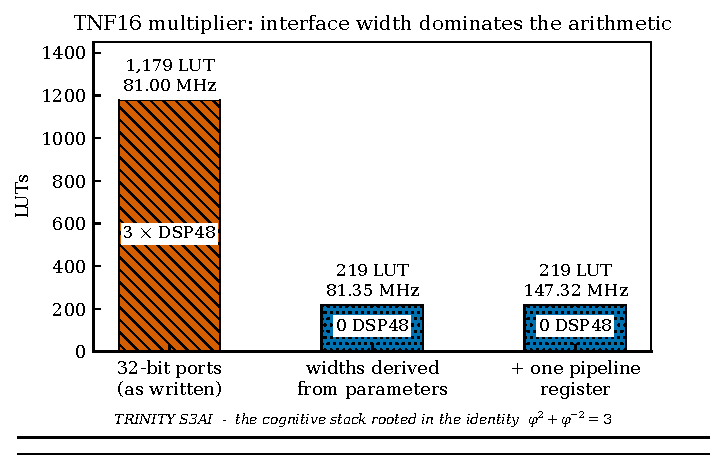
\includegraphics[width=\columnwidth]{tnf_width.pdf}
\caption{The same arithmetic at three interface widths.}
\label{fig:width}
\end{figure}

\subsection{The same width decided correctness}
At TNF32 the significand product needs 52 bits. The 32-bit wire truncates, and
the module returns wrong results while appearing to support the rung, since its
own documentation names TNF32 as a supported configuration. Measured against a
64-bit reference: 1{,}995{,}730 mismatches in 2{,}128{,}964 combinations.

Deriving every width from the format parameters removes both problems at once. We
report this because the pattern is not specific to TNF: in a parametric
arithmetic core, a width that is merely \emph{large enough for the configuration
that was tested} is a silent-truncation trap at the next one, and it will not be
caught by a testbench written against the tested configuration.


% ---- tnf_paper.tex lines 6322-6398: What the formal statements are, and what they are ----
\section{What the formal statements are, and what they are
not}\label{sec:statusofstatements}

This paper carries a large number of numbered statements, and they are not all the
same kind of object. Collecting the distinction in one place is a service to a
reader who wants to know which lines could be wrong for a mathematical reason and
which could be wrong for an empirical one.

\paragraph{Three kinds of statement.} The first kind is \emph{analytically
proved}: it follows from arithmetic, from the irrationality of $\log_2 3$ or
$\varphi$, or from an algebraic identity, and no measurement can disturb it.
The economy theorem, the no-free-lunch theorem,
the packing-density theorem, the Lucas-trace theorem,
the $\varphi$-rounding-envelope lemma, the $\varphi$-ratio bound and
\extended{the negative-product proposition} are of this kind. The second kind is a
\emph{proposition about a model}: it is a correct deduction from a cost model,
error model or workload assumption that is itself an idealisation, so it is exactly
as reliable as the model it is stated over --- the $\kappa$ statements and the
width-rule optimisations belong here, and the way for them to fail is for the
model to be the wrong model, not for the algebra to be wrong. The third kind is an
\emph{empirical observation} stated in numbered form for reference: post-route
resource and frequency figures, perplexity comparisons, and error measurements
over sampled distributions. These can be falsified by rerunning them, and the
places where our own earlier runs were falsified in exactly this way are recorded
in Section~\ref{sec:limitations-anchor} and in the erratum discussion.

\paragraph{Eight conclusions this work supports.} The following are the load-bearing
conclusions, each with the status it actually has.

\begin{enumerate}
\item The $\varphi$ split has a \emph{finite-width} certificate and not only an
asymptotic one: for $e\geq1$ the deviation of $m/e$ from $\varphi$ is strictly
below $\varphi^{2}/(2e)$ (\extended{the $\varphi$-ratio bound}). The residual can
therefore be reported at a given width rather than promised in a limit
[proved].

\item The exact coefficient $\varphi^{-2}$ never produces an ambiguous rounding at
any non-zero width (\extended{the $\varphi$-rounding-envelope lemma}); every tie-breaking
ambiguity in circulation comes from a truncated decimal surrogate for the
coefficient, and first bites at $N=12{,}239$ [proved].

\item Packing a ternary exponent into bits is not merely lossy: the count of
unreachable codes is positive and odd at every trit budget, and the utilisation
visits a dense subset of $(1/2,1)$, so no tail of the ladder is asymptotically
efficient (\extended{the packing-density theorem}) [proved].

\item Even powers of $\varphi$ admit an integer-only certificate through
$S_{n+2}=3S_{n+1}-S_n$ (\extended{the Lucas-trace theorem}), which makes a depth-$k$
$\varphi$-stack auditable with no rounding model in the loop. This is a testability
result, not an accuracy claim [proved].

\item One additional ternary exponent position multiplies the scale-state count by
three and halves the significand cell count. That exchange rate is exact and it is
the whole content of the static split [proved].

\item Objectives of the form $R^{a}P^{b}$ never select an interior split
(\extended{the negative-product proposition}). The $\varphi$ rule therefore cannot
honestly be presented as the maximiser of a range-times-precision product, and
this paper does not present it as one [proved --- negative result].

\item The new ratio bound was additionally checked by exhaustive integer
enumeration at every $N=4,\dots,100{,}000$ with no violation. This is a
sanity-check on the proof, not a substitute for it [measured].

\item An objective that could justify the $\varphi$ split for a specific workload
would have to carry the value distribution, the overflow policy and a hardware
cost model. No such objective is derived here, and constructing one is left open
[open].
\end{enumerate}

\paragraph{Two facts that constrain rather than support the design.} Etiemble's
argument that three is not the optimal radix for computation~\cite{etiemble2019} is
accepted here on its own terms, and the microscaling study showing that finer
granularity is not monotonically better~\cite{fasoli2026} bounds how far any
scale-grid refinement can be expected to go. Both are cited above at the points
they bear on, and neither is treated as a matter of opinion.


% ---- tnf_paper.tex lines 6209-6321: Adjacent work this paper is measured against ----
\section{Adjacent work this paper is measured against}\label{sec:adjacent}

Four bodies of work published while this paper was being prepared bound its
claims, and each is named here rather than left to a reader to supply.

\paragraph{The standards baseline.} The binary baselines used throughout ---
\texttt{binary16}, \texttt{binary32}, \texttt{binary64} --- are the ones defined
by IEEE Std 754-2019~\cite{ieee754_2019}, and the eight- and four-bit baselines
are the ones being fixed by the IEEE P3109 working
group~\cite{p3109wg2026}. The 83-format catalogue this work draws its
conformance vectors from cross-walks against P3109 explicitly~\cite{catalogue}.

\paragraph{Two independent machine-checked treatments of the nearest standard.}
P3109 arithmetic has been formalised twice and independently: in Imandra/IML,
presented at ARITH 2025~\cite{wintersteiger2025}, and in Lean, as
FLoPS~\cite{flops2026}. This bounds the claim this paper makes about
auditability. Bit-exact conformance vectors establish determinism of a decode
and arithmetic law against an independent oracle; when the same vectors are
replayed on a board, and the bitstream fingerprint, the device identifier and the
transcript are archived together, they establish determinism \emph{on that part}.
A mechanised proof establishes semantics instead. These are different layers, and
this work supplies conformance in the reported open flow, not a mechanised
semantics. The gap between those layers is narrowing and it should be said so:
formally verified \emph{synthesizable} floating-point data types have now been
demonstrated inside an HDL~\cite{archhdl2026}, which moves machine-checked
guarantees from the model down to the register-transfer description that gets
synthesised, and the broader formal-verification effort for floating-point
arithmetic continues independently of the P3109 track~\cite{mohanty2025}, while
the cost of applying formal tools to register-transfer code is itself falling, with
open-source multi-agent pipelines now reported for formally checked RTL
repair~\cite{tran2026rtlrepair}, and an executable hardware-intent layer has been
proposed to make microarchitectural obligations explicit before RTL lowering
and synthesis~\cite{cheng2026hint}. Against
that, a conformance transcript replayed on a specific part is not a weaker proof
of the same thing but a different object: it is evidence about a physical device
and its bitstream, which a proof about an HDL description does not provide, and it
is silent about semantics, which the proof does provide. This paper claims only
the former. The same line of
work also supplies $\kappa$-approximation~\cite{fitzgibbon2026kappa}, a
scale-invariant accuracy measure on the standards track; the error figures
reported here are mean relative error over exact rationals and are not
$\kappa$-approximation figures, and should not be read as such.

\paragraph{Bit-exactness as an audit primitive.} The use this paper makes of
conformance vectors --- a reproducible fingerprint of an arithmetic law --- is the
same primitive being developed for inference auditing, where bitwise-precise
re-computation is shown to be achievable without a performance
penalty~\cite{cankaya2026}. That line supports the value of the primitive and
must not be conflated with a different sense of determinism, obtained by
scheduling and verified speculation over arithmetic that is itself not
bit-reproducible~\cite{gond2026llm42}. The two are separate layers, and only the
first is what a format can supply. The distinction is not academic: a 2026 study
locates the numerical instability of large-model inference in the arithmetic and
the reduction order rather than in the schedule, and has to intervene at that
level to obtain reproducible output~\cite{zhu2026heal}, which is evidence that the
layer a format governs is the binding one. The first layer is also acquiring load-bearing
applications rather than only audit arguments: byte-exact reuse of cached
intermediate state across models has been used as the correctness condition of a
knowledge-transfer pipeline~\cite{schelpe2026grafting}, where a single differing
byte invalidates the construction. Whatever one makes of the pipeline, it is an
instance of bit-exactness being consumed as a contract rather than reported as a
virtue, which is the direction that makes a conformance ledger worth publishing.

\paragraph{Earlier combinations of tapering and a non-standard radix.} The
tapered-precision route is older and wider than the posit and takum line cited
above: a tapered floating-point extension has been proposed for the redundant
signed radix-2 system via canonical recoding~\cite{schoenbaum2021}, which is a
prior combination of tapering with a non-standard digit set and is acknowledged
here as such. The takum line has meanwhile been evaluated outside machine
learning, in sparse linear solvers against bfloat16 and posit~\cite{hunhold2024sparse},
which is the closest thing available to an independent accuracy baseline for
tapered formats and is the reason no accuracy superiority over takum is claimed
in this paper.

\paragraph{Accuracy is not a property of the field layout alone.} Matsuoka's
two-part argument~\cite{matsuoka2026fp8a,matsuoka2026fp8b} separates
\emph{precision} --- the native width of the format --- from \emph{accuracy},
recovered by the accumulation strategy, with Kulisch fixed-point accumulation as
the escape route. That separation supports the position taken here that the
$\varphi$ rule is a rule for choosing fields and not a different arithmetic, and
it also limits it: no field layout at sixteen bits removes the need for a wider
accumulator. The comparative picture across INT and FP at fine granularity is
surveyed for the same generation of formats in~\cite{int_vs_fp2025}, and the
performance--efficiency trade-off for low-precision formats was mapped
earlier in~\cite{mlformats}.

\paragraph{A direct threat to the representation--computation separation.}
CurveFP is a recent and materially different warning against over-generalising
the separation used in this paper: it co-designs a block-scaled,
logarithmic representation with a closed product operation, and reports
downstream language-model results together with a preliminary accelerator-tile
area result~\cite{qiao2026curvefp}. We therefore mark it as
\textbf{[threat]} to any claim that a representation-level observation is
unlikely to transfer to computation. It is not a head-to-head comparison with
TNF: CurveFP uses block scales and interleaved logarithmic curves, whereas TNF
uses a fixed ternary-derived field split, and the result record is a preprint
with a different workload and hardware model. The conclusion supported here is
narrower: our own TNF evidence must be stated as task- and rung-specific, and
the conjugate-gradient table above is not evidence about language-model
training, product closure, area, or energy. A direct CurveFP--TNF experiment
remains open.

\paragraph{Contemporaneous ternary and alternative-format hardware.} Ternary
inference hardware on FPGA is an active line independent of this
one~\cite{tereffic2025,tenet2025}, although it ternarises \emph{weights} rather
than the number representation. Posit arithmetic has been evaluated on FPGA and
GPU accelerators with quantified logic overhead~\cite{posit_accel2024}, and
logarithmic number systems have been co-designed with LLM datapaths on
FPGA~\cite{pnnl_lns2025}; both are baselines in the tables above. Uses of the
golden ratio in computing have been surveyed
systematically~\cite{akhtaruzzaman2024phi}, and the present rule should be read
against that survey rather than as an isolated idea.


% ---- tnf_paper.tex lines 7627-7758: Limitations ----
\section{Limitations}\label{sec:limitations-anchor}\label{sec:limits}

\paragraph{The fabric this format is optimal on does not exist to buy.}
\extended{the no-free-lunch theorem} confines the ternary encoding's benefit to a ternary
fabric, and no such process is commercially available. Every hardware figure in
this paper is therefore a post-route estimate for binary FPGA fabric, where the
ternary exponent neither gains nor loses on the scale-state count --- the
enumeration in \extended{the enumeration section} shows it ties a binary encoding
exactly at the widths tested. It does lose on a second axis, and this revision
proves it: \extended{the range-per-bit theorem} shows a ternary exponent never buys range
per stored bit, with equality only at $t=1$. The two statements are about
different axes and both hold. The claims that survive on parts you can buy today are the fixed-field
ones: no regime codec, no exponential to
evaluate. The ternary claim is architectural and is labelled as such throughout.

\begin{enumerate}[leftmargin=*]
\item \textbf{The comparison was against takum16, not tekum16 --- and the
genuine tekum comparison has since been done.} The oracle labelled tekum
decodes all $65{,}536$ 16-bit codes identically to the takum oracle; it is a
linear binary model of takum's layout. \texttt{tekum\_true\_ref} now
implements the real base-3 tekum of arXiv:2512.10964, Definitions 7--8 --- the
paper's worked example reproduces exactly and the encoding is monotone on all
$6{,}559$ tekum8 codes. Its widths count trits, so tekum16 is 16 trits
$= 25.4$ bits with $3^{16}$ codes. At equal stored width the accumulation
benchmark is a three-way tie: tekum10 ($15.85$ bits) $8.56\mathrm{e}{-3}$,
takum16 $5.70\mathrm{e}{-3}$, TNF(4,8) $5.32\mathrm{e}{-3}$ at the 16-bit
class, and $1.43/1.26/1.20\mathrm{e}{-7}$ at 32. No format wins by more than
the width it gives up.

\item \textbf{The reference oracle carried a sign defect, now fixed.} Round-tripping
$1.5$ through the parameterised oracle returned $-1.5$ at mantissa widths of 21
and 25 bits: the sign bit sat at a fixed position while the exponent mask took
more bits than the field holds, so the two overlapped. Both are now derived from
the format parameters, and TNF32's round-trip error falls from
$5.4\mathrm{e}{-1}$ --- what a systematically inverted sign averages to --- to
$5.3\mathrm{e}{-9}$.

We record how it survived, because the lesson outlives the bug. The ladder's
check was add/mul commutativity, and an inverted sign survives on both sides of
$a+b=b+a$. The check was real and blind to the class. A round-trip assertion sees
it, costs one line per probe, and now runs at all nine rungs. tekum~\cite{tekum} is a descendant of takum~\cite{takum} adapted for balanced
ternary. Our
linear oracle reconstructed it from takum's field scheme; the full per-trit
specification is now implemented from the tekum paper as
\texttt{tekum\_true\_ref} (Definitions 7--8, exact on the worked example,
monotone on all $6{,}559$ tekum8 codes). The takum oracle carried a defect of
its own --- negation flips the exponent sign, and every negative code decoded
wrongly until \#606; it now matches libtakum on $65{,}534$ of $65{,}535$ codes
--- so every takum ratio measured before that fix is superseded by the
equal-width tie of \extended{the accuracy section}.

\item \textbf{The head-to-head in hardware now exists, with caveats.} takum's
published codec RTL is VHDL~\cite{takumrtl} and was not synthesised here, so
those figures remain TNF's own. What has since been synthesised head-to-head:
\texttt{tef\_add\_full} --- sign, subtract, round-to-nearest-even, normalise
--- verified on $3{,}000$ oracle vectors plus $40$ chained accumulations of 32
terms with zero errors, at $397$ LUT / $45$ CARRY4 for TNF(4,8) against
$1{,}182$ LUT / $211$ CARRY4 for a 16-bit adder of the \emph{linear
takum-layout model}, $2.98\times$; and the first real-tekum hardware,
\texttt{tekum8\_decode.v}, exhaustively verified on all $6{,}558$ codes with
zero errors, at $542$ LUT / $96$ CARRY4 against $1$ LUT for the TNF
field-slice decode. Caveats, all of them: Yosys 0.65 \texttt{synth\_xilinx},
last stat block only (an earlier extraction summed all blocks and inflated
every figure threefold), post-synthesis with no place-and-route and no board;
the adder competitor is a structural model of takum's layout, not the
published VHDL; and on a ternary fabric tekum's trit extraction would be
wiring. What is visible in that source, and what we report as structure
rather than measurement, is this: the 16-bit codec instantiates a 725-line
generated leading-zero counter and barrel shifter --- machinery a fixed-field
format does not need for regime decoding.

\item \textbf{The range is bounded} at $\pm39$ in powers of two, roughly $\pm12$
decades, where a regime field is unbounded. Fixed fields buy the cheap datapath
and the uniform mantissa; range is the price, and workloads that need more should
raise the trit budget or use a tapered format.

\item \textbf{Accuracy above TNF32 requires exact rationals, and now uses them.}
Once the oracle defect was fixed, TNF32 measures $5.17\mathrm{e}{-9}$, flat
across the workload, which is what 25 mantissa bits should give. TNF64 carries
52 mantissa bits in the research note --- 56 once the width rule is applied ---
and 52 is exactly the significand of the IEEE double, so a double-precision
metric at that rung and above would describe the metric rather than the format.
\extended{The value-law table} is therefore computed in exact rationals with 1{,}200-bit
significands, which is what lets the upper rungs be quoted at all; the hardware
limit below is separate and unchanged.

\item \textbf{Five of nine rungs have post-route implementation results.} TNF4 through TNF64 fit
the device, TNF64 at $7{,}479$ LUTs and $48.20$\,MHz. TNF128 at its reconciled
$M = 119$ does not
converge in routing on this part and is not claimed; TNF256 upwards exceed a
single Artix-7 fabric entirely. \extended{The specification table} is the specification at the
width rule; \extended{the routed-ladder table} is what was placed and routed. We keep them
apart on purpose.

\item \textbf{The shipped reference oracle is still on the research-note widths.}
The published \texttt{tnf\_ref.py} ladder table carries $(E_t,M)$ of
$(4,9)$, $(5,21)$, $(7,52)$, $(8,115)$ and upward --- the pre-reconciliation
budgets, seven of which do not satisfy $1+E_t+M=N$ --- an earlier revision of this
item said three, and the per-rung audit in \extended{the ladder-version table} says
seven. \extended{The specification table} above is
the reconciled specification, not a transcript of that file. Bringing the oracle
onto the width rule changes its conformance vectors and therefore their SHA-256
fingerprints, so it is a versioned change and is not folded in silently here.
\extended{The variant-A section} describes how that versioning was carried out: both
ladders now ship as named objects with hash-pinned vector manifests, so the
research-note configuration stays reproducible instead of being overwritten. Any
figure in this paper that quotes an oracle result quotes the research-note
configuration it was actually run at, and the two must not be cited as one
artefact.

\item \textbf{One device family.} The results use Artix-7 on an open flow; they
are not a multi-corner characterisation, and an ASIC mapping will differ.

\item \textbf{The ternary-fabric argument is architectural.} No ternary process
exists to synthesise on. \extended{The hardware section} is a binary-fabric result;
the ternary claim is reasoning about regime decode and native exponent addition
and should be read as such.
\end{enumerate}
% ---- tnf_paper.tex lines 7759-7786: Reproducibility ----
\section*{Reproducibility}

The reference oracle, the RTL, the equivalence testbenches and the synthesis
commands are public. The toolchain is Yosys 0.65, nextpnr-xilinx 1743d0f,
Icarus Verilog 13.0 and Python 3.14 --- all open-source, none requiring a
licence, which is the point: a result nobody can reproduce without buying
something is not a public result.
\section*{Disclosure}

An AI coding assistant was used in preparing the software, the measurements'
tooling and this manuscript. Every figure reported here was produced by running
the named tools on hardware in the author's possession. Figures from that
toolchain are reported as post-route estimates, and where a figure is derived rather than observed it is
labelled.

